
\chapter{Introduzione}\label{capitolo1}


\section{Introduzione}

da fareÈ


\section{Animazione e Simulazione}

A partire dagli anni '80, lo sviluppo di animazioni per la visualizzazione
di algoritmi è stato in continuo aumento. Una tra le prime testimonianze
che si ha di questo fenomeno è {}``Sorting out sorting'' \cite{video},
un video di presentazione degli algoritmi di ordinamento, una novità
nel suo genere.

Dal 1981 fino ad oggi, le rappresentazioni di algoritmi e strutture
dati si sono diffuse ed hanno trovato il loro principale utilizzo
come supporto per studenti ed insegnanti nei relativi corsi universitari.

Osservando il materiale disponibile ad oggi sul web e come ci fa notare
\cite{MatrixPro}, possiamo riconoscere che esistono principalmente
due direzioni in cui si sono sviluppati i programmi di AV (Algorithm
Visualization): l'animazione e la simulazione.La prima consiste in
una visualizzazione degli effetti che un predefinito algoritmo ha
su una struttura dati creata dal programmatore; l'utente, in questo
caso, assiste passivamente all'animazione osservandone i risultati
sulla struttura dati. Nel secondo caso parliamo di simulazione, in
quanto l'utente manipola gli oggetti messi a disposizione dal programmatore
secondo le operazioni permesse dalla struttura, in modo da creare
una sequenza di passi analoghi a quelli dell'algoritmo che si sta
analizzando.

Naturalmente questa è una classificazione grossolana, in quanto ogni
software possiede proprie particolari caratteristiche. Le funzionalità
introdotte negli anni nelle varie applicazioni disponibili, hanno
permesso una seconda classificazione più accurata, definita in base
all'interazione che tali visualizzazioni permettono agli studenti.
Il risultato del gruppo di lavoro su {}``Improving the Educational
Impact of Algorithm Visualization'' (Giugno 2002, ITiCSE, Denmark)
è stata la suddivisione in sei categorie delle tecniche di insegnamento
classificate in base al supporto di visualizzazione utilizzato (riportata
in \cite{AV-compare}): 
\begin{enumerate}
\item Nessuna visualizzazione (No viewing), gli studenti non hanno a disposizione
nessun supporto visivo, o solamente immagini non animate, illustrazioni
del libro;
\item Visualizzazione (Viewing), osservazione passiva dell'esecuzione dell'algoritmo,
in cui possibile in alcuni casi controllarne il flusso di esecuzione
tramite comandi di avanti - indietro;
\item Rispondere (Responding), come per il punto precedente, consiste nell'osservazione
della rappresentazione animata dell'algoritmo, durante la quale allo
studente è richiesto di rispondere ad una serie di domande, o svolgere
esercizi su carta, relativi all'argomento presentato;
\item Cambiare (Changing), modificare la visualizzazione principalmente
attraverso la personalizzazione dei dati in ingresso dell'algoritmo,
in modo da analizzare il comportamento dell'algoritmo nei vari casi
testati;
\item Costruire (Constructing), costruire la propria animazione di un particolare
algoritmo che si sta studiando con l'aiuto fornito dai programmi messi
a disposizione;
\item Presentare (Presenting), pianificare lezioni nelle quali gli studenti
debbano presentare ad un pubblico la visualizzazione di un particolare
algoritmo, possibilmente creata da loro secondo il punto 5, per poi
procedere ad una discussione sull'argomento. 
\end{enumerate}
I risultati ottenuti delle diverse tipologie di insegnamento appena
riportate sono oggetto di numerosi studi presenti e passati, e una
sintesi dei dati raccolti è presente nella sezione \ref{sec:studi-effettuati-sull'efficacia}.


\section{\label{sec:studi-effettuati-sull'efficacia}Utilizzo di AV nell'insegnamento}

A seguito della classificazione delle tipologie di insegnamento dei
corsi riguardanti Algoritmi e Strutture Dati, e la loro interazione
con le tecnologie di visualizzazione algoritmi, sono stati effettuati
numerosi studi a proposito dell'efficacia dell'introduzione di queste
nuovi metodi sull'apprendimento degli studenti.

Un'analisi generale è riportata in \cite{AV-compare}. Lo studio \cite{byrne}
ha riportato che gli studenti analizzati che hanno utilizzato un supporto
alle lezioni di tipo 3(responding) e 5(construction), hanno ottenuto
risultati migliori nei test, rispetto ad altri studenti che non ne
avevano fatto uso, o che avevano utilizzato una semplice animazione
(livello 2). I risultati sono però in conflitto con quelli raccolti
nello studio \cite{jarc}. Secondo quest'ultimo, non è stata evidenziata
alcuna differenza significante nei risultati agli esami ottenuti dagli
studenti con l'una o l'altra tipologia di supporto alle lezioni.

L'analisi i cui risultati sono riportati in \cite{AV-compare}, mette
in risalto il miglioramento degli studenti, in base alla tecnica di
supporto interattivo utilizzata, tenendo anche in considerazione le
conoscenze precedenti dei soggetti riguardo l'argomento affrontato.
I soggetti, provenienti da 3 diverse università, sono stati messi
a confronto con un pre-test, nel quale venivano valutate le loro conoscenze
e attitudini, prima di affrontare le lezioni. A seconda dei risultati,
sono stati divisi in tre gruppi, e per ognuno dei quali sono state
effettuate una serie di incontri sull'argomento degli algoritmi di
ordinamento con l'utilizzo di 3 diversi metodi: 
\begin{enumerate}
\item Lezioni frontali senza supporti visivi. Gli studenti di questo gruppo
sono stati quelli che hanno ottenuto un punteggio alto nel pre-test,
ovvero erano i soggetti con maggiori conoscenze e potenzialità;
\item Lezioni frontali con l'utilizzo da parte del docente di una presentazione
in lucidi e di un tool di visualizzazione di algoritmi;
\item Lezioni frontali (come per il gruppo 2) con l'aggiunta di ore supplementari
nelle quali si svolgeva l'attività di laboratorio, in cui gli studenti
avevano la possibilità di utilizzare singolarmente un'applicazione
(JHAVÈ \cite{JHAVE}) che permette di osservare l'animazione degli
algoritmi, integrata con domande ad-hoc. 
\end{enumerate}
A seguito di queste attività, gli studenti sono stati esaminati con
un test di verifica uguale per tutti i gruppi.

I risultati ottenuti si sono rilevati concordi con \cite{byrne} in
quanto, rapportando le conoscenze iniziali degli studenti con gli
esiti dei test di verifica, si è osservato che maggiore è stata l'interazione
con lo strumento di supporto, maggiori sono stati i progressi ottenuti
dai soggetti.

Con i risultati ottenuti in questa ricerca, si è quindi potuto concludere
che i risultati non significativi di \cite{jarc} fossero dovuti ad
un'inadeguata tecnica di raccolta: nel caso delle domande, gli studenti,
lasciati liberi a se stessi e non confinati in un laboratorio, hanno
affrontato l'attività come un gioco e non come uno strumento educativo.
Sottoponendoli ad una maggiore concentrazione in un lasso di tempo
determinato e ristretto, i soggetti dello studio \cite{AV-compare}
hanno invece ottenuto risultati positivi.

Per quanto riguarda i programmi della categoria 6 (presentig), non
sono purtroppo ancora presenti studi che indichino l'efficacia di
tale tecnica di insegnamento.

Sono inoltre presenti testimonianze di corsi universitari di Algoritmi
e Strutture dati \cite{course} in cui le tecniche di visualizzazione
di algoritmi sono state integrate completamente nel programma di studi.
Si è inoltre verificato che gran parte degli studenti che hanno partecipato
alle lezioni del corso, hanno superato l'esame fin dal primo appello.


\section{Come creare un buon AV}

Algoviz \cite{wikiAlgoViz} costituisce il sito di riferimento per
studenti, docenti e chiunque altro sia interessato nella ricerca di
un'applicazione che raccolga visualizzazioni di algoritmi, o l'animazione
di una particolare struttura. Dal 2006 il sito cataloga in un proprio
archivio (aggiornato settimanalmente) tutte gli strumenti rintracciabili
sul web relativi a questo argomento. Tale sito è stato anche il punto
di partenza di questa tesi, in quanto ha permesso di esplorare e analizzare
i principali pacchetti software per sviluppatori presenti al momento,
ed inoltre contiene un'interessante guida dedicata a chi si appresta
a realizzare una propria visualizzazione di algoritmi.

Si riporta ora una sintesi dei principi chiave esposti nella guida: 
\begin{description}
\item [{{Coinvolgere}}] fare in modo che l'utente partecipi attivamente
durante l'animazione dell'algoritmo, evitando le presentazioni statiche
e passive;
\item [{{Semplificare}}] ridurre la complessità dell'applicazione, a
partire dall'interfaccia grafica. Per quanto riguarda l'esposizione
dei concetti, nascondere per quanto possibile i dettagli implementativi
degli algoritmi, ed animare i singoli passi per le operazioni più
complesse. L'applicazione inoltre deve essere talmente semplice da
aver bisogno di una documentazione minima relativa al proprio funzionamento,
poichè l'utente deve riuscire ad avviarla e comprenderne l'utilizzo
fin dal primo avvio;
\item [{{DataSet}}] fornire diverse tipologie di gestione dei dati in
ingresso

\begin{itemize}
\item Dati inseriti dall'utente, per permettere l'eplorazione di tutte le
possibili configurazioni, dando la possibilit allo studente di verificare
il comportamento della struttura in casi particolari da lui costruiti; 
\item Dati random, di cui l'utente potrebbe controllare solo alcuni parametri
(con la dimensione, il range, ecc..); 
\item Dati pre-costruiti ad hoc, che permettano allo studente di analizzare
il comportamento chiave dell'algortimo in situazioni chiave, preparate
ad hoc dal docente o dal programmatore. Questa funzionalit risulta
utile perch generalmente gli studenti (soprattutto se alle prime armi)
non ha la fantasia necessaria per creare casi particolari di testing. 
\end{itemize}
\item [{{Controllo}}] se si tratta di una semplice rappresentazione animata
dell'esecuzione di un programma su di una struttura dati, è fondamentale
permettere allo studente di controllare il flusso dell'animazione
attraverso una serie di comandi, come la gestione della velocità (nel
caso si parli di un'animazione continua), la possibilità di procedere
passo-passo e di andare avanti e indietro nell'animazione. Algoviz
riporta che l'utilizzo dell'animazione spezzata in passaggi, riscontra
risultati migliori nell'apprendimento rispetto ad una visualizzazione
continua delle azioni. 
\end{description}

\section{\label{sec:Strumenti-Disponibili}Strumenti Disponibili}

La relazione \cite{AlgoViz} redatta dal gruppo di lavoro di Algoviz,
illustra il lavoro di raccolta di AV da essi realizzato nel 2006:
sono stati trovati circa 350 AV all'epoca, che quindi sono stati raccolti
e classificati all'interno del catalogo presente nel sito aggiornato
settimanalmente. Ad oggi contiene più di 500 visualizzazioni. Gran
parte degli strumenti catalogati riguarda gli argomenti principali
affrontati nell'insegnamento di Algoritmi e Strutture dati, primo
fra tutti il problema dell'ordinamento, al quale seguono le strutture
di ricerca (Alberi Binari di Ricerca in particolare), le strutture
lineari e gli algoritmi che operano sui grafi.

A partire da questa raccolta, si sono analizzati i principali pacchetti
che potenzialmente costituivano un punto di partenza per altri sviluppatori,
dal quale partire per creare la propria applicazione di animazione
di algoritmi. Gran parte delle applicazioni raccolte consistono in
passive rappresentazioni di algortimi che agiscono su strutture dati
preinstallate (quindi non personalizzabili) durante le quali l'utente
coinvolto solo per quanto riguarda il controllo del flusso. Esistono
però alcune eccezioni, in cui tale rappresentazione viene arricchita
con funzionalità interessanti che catturano e focalizzano meglio l'attenzione
dello studente sull'argomento.

Di seguito sono descritti alcuni dei principali pacchetti che sono
stati analizzati durante la ricerca. Molti altri software sono stati
esaminati, ma in questa circostanza non sono riportati, poichè sono
risultati presentare caratteristiche molto simili a quelle dei programmi
che ora verranno introdotti. 
\begin{description}
\item [{{Animal}}] Il software Animal \cite{Animal} è un'applicazione
java che permette di osservare l'animazione di un particolare problema,
corredata da un'adeguata e ricca documentazione (anch'essa animata)
sull'argomento affrontato. Nel pacchetto si trovano pre-installate
diverse presentazioni. L'utente ha comunque la possibilità di creare
la propria animazione. In questo caso si offre al docente la possibilità
di arricchire le proprie lezioni frontali con presentazioni animate
dell'algoritmo.
\end{description}
\begin{figure}[htbp]
\centering
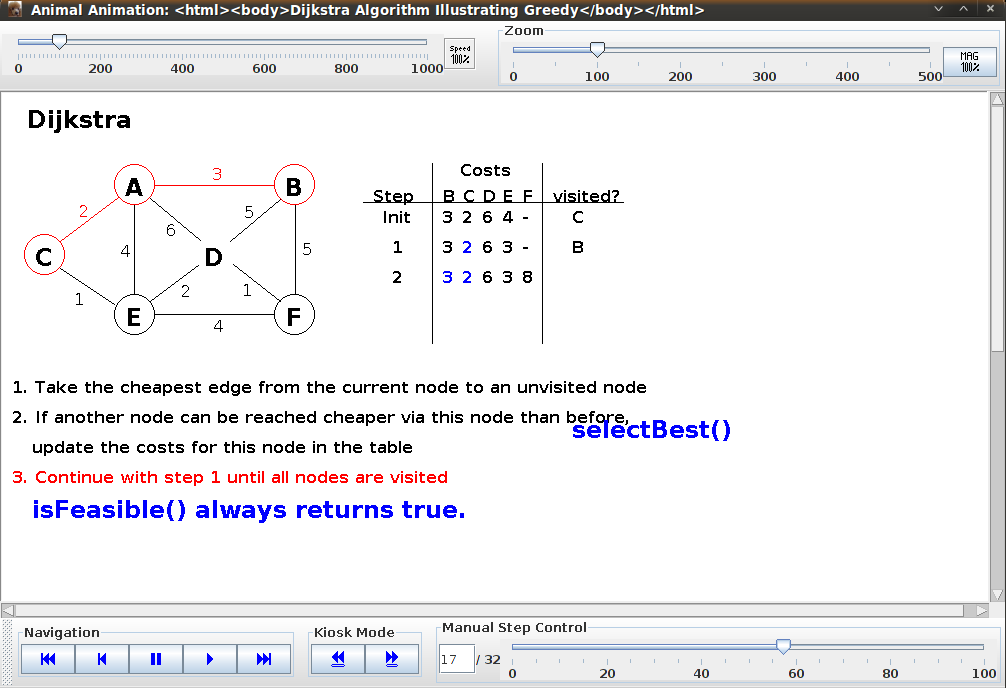
\includegraphics[scale=0.25]{images/Animal_screenshot.png}
\caption{Screenshot di Animal}
\end {figure}
\begin{description}
\item [{{JHAVÈ}}] è un'applicazione web, le cui presentazioni sono salvate
all'interno di parcticolari server. Apparentemente molto simile ad
Animal, JHAVÈ offre allo studente una serie di funzioni aggiuntive
molto interessanti, che ne migliorano sicuramente il coinvolgimento.
Tra queste troviamo per prima cosa la scelta del tipo di dati in ingresso
desiderati: generati casualmente dal programma, o inseriti personalmente
dall'utente. Come per Animal l'animazione è ben documentata, in questo
caso con l'aggiunta dello pseudocodice relativo all'algoritmo. Inoltre,
l'animazione è interrotta (con frequenza variabile) da domande in
linea con l'argomento affrontato che coinvolgono direttamente i dati
inseriti per l'animazione. Lo studente è invitato a rispondere alle
domande per poter proseguire nell'animazione. Date le sua caratteristiche,
si può concludere che JHAVÈ si colloca a livello 4 (changing) nella
catalogazione delle visualizzazioni.
\end{description}
\begin{figure}
\centering
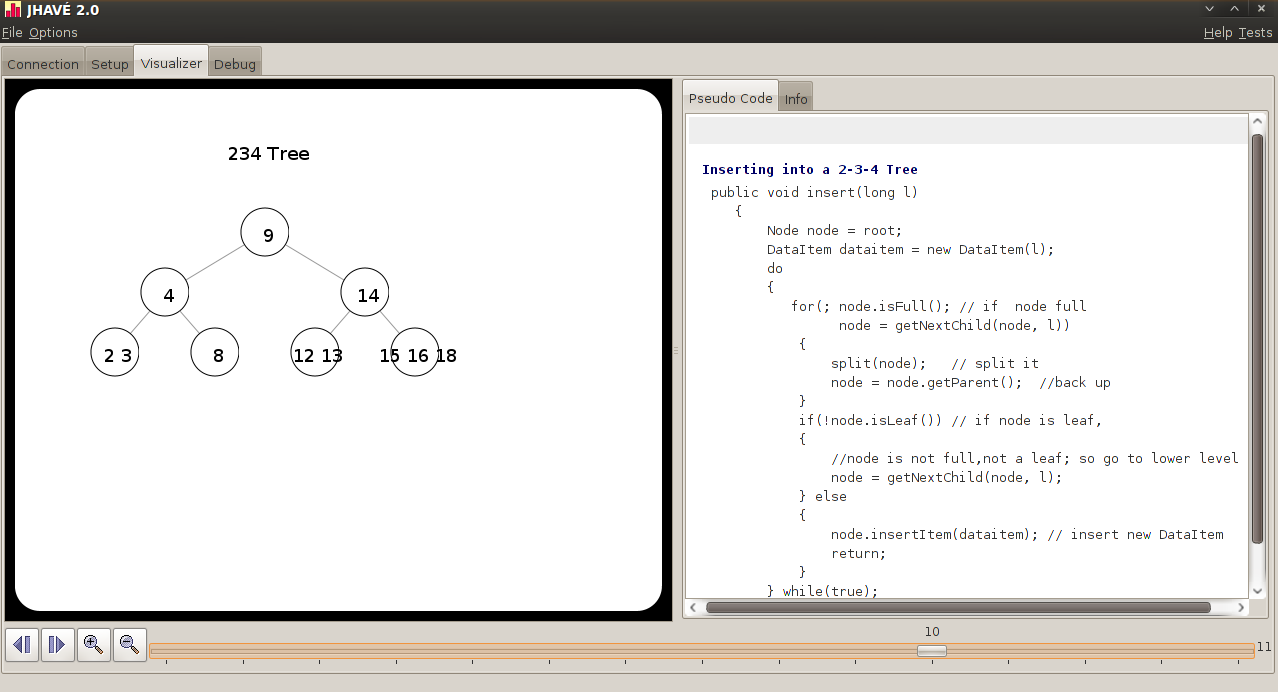
\includegraphics[scale=0.25]{images/JHAVE_screenshot.png}
\caption{Screenshot di JHAVE}
\end{figure}
\begin{description}
\item [{{MatrixPro}}] e Trackla2. Il software dalle funzioni più interessanti.
Si colloca a livello 5 (constructing). Le sue caratteristiche sono
descritte in maggiore dettaglio nel capitolo seguente.
\end{description}

